\chapter{Experiments}
In this section, I will discuss how I evaluate the LSH with some real world data, and comparison with other spatial indexes. Finally, present the outcome that is measured from various aspects.

\section{Experimental Setup}

For evaluation, the LSH is implemented in C++ and has been tested on a machine with 2.2GHz 6-core Intel Core i7 CPU and 16GB memory. 

\begin{center}
\begin{adjustbox}{max width={\textwidth}, max totalheight={\textheight},keepaspectratio}
\begin{threeparttable}
\caption{Datasets}

\begin{tabular}{c|c c c}
    \toprule
                        % & \multicolumn{3}{c}{Dataset} \\\midrule \midrule
    \textbf{Name}    &\textbf{Size}  & \textbf{No. of data pairs} & \textbf{Data type}             \\ \midrule 
    \texttt{post}    & 2.2M & 123,593             &Geographic Coordinates \\
    \texttt{g2}      & 18K  & 2,048               & Synthetic Clusters    \\
    \texttt{osm}     & 3.0G & 114,932,854         &Geographic Coordinates \\
     \bottomrule
\end{tabular}
% \begin{tablenotes}
% \item[1] qwerty; \item[2] asdfgh
% \end{tablenotes}
\end{threeparttable}
\label{table:datasets}
\end{adjustbox}
\end{center}

\textbf{Datasets}: As shown in the Table \ref{table:datasets} above, we have two real world datasets the \texttt{post} \cite{rtreeportal} and \texttt{osm} \cite{OpenStreetMap}, and one synthetic dataset the \texttt{g2} \cite{G2sets}.

\begin{itemize}
  \item \texttt{post}: The \texttt{post} dataset contains 123,593 coordinates of post offices across North America. The distribution of this dataset is more evenly.
  \item \texttt{g2}: The \texttt{g2} is a synthetic cluster dataset that contains 2,048 points that are computed from Gaussian clusters with 2 dimensions and the standard deviation set to 10. 
  \item \texttt{osm}: The dataset \texttt{osm} contains 114,932,854 coordinates in Australia and Oceania from OpenStreetMap. This dataset contains large amount of data points, and its distribution is highly skewed. 
\end{itemize}


\begin{figure}
    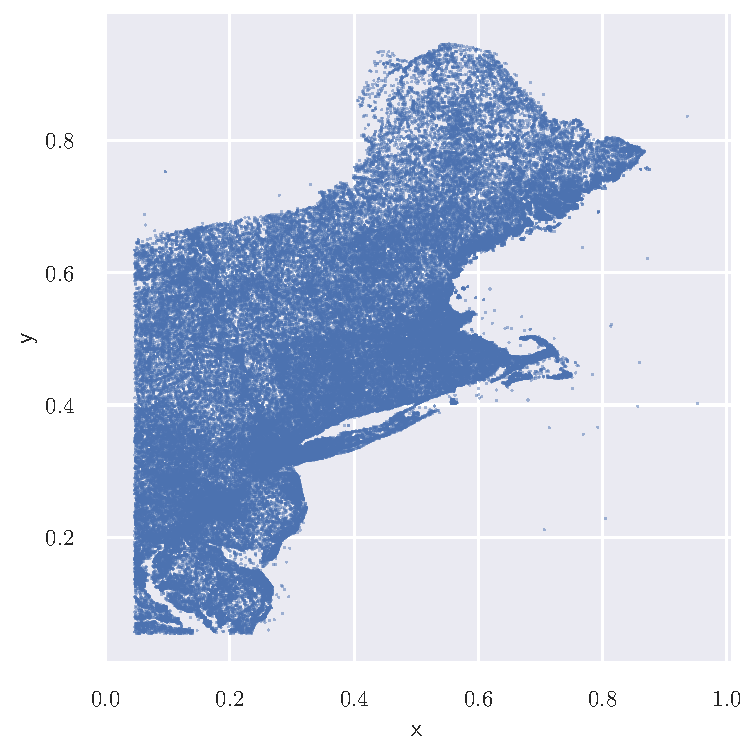
\includegraphics[width=.33\textwidth]{Figures/post_p.pdf}\hfill
    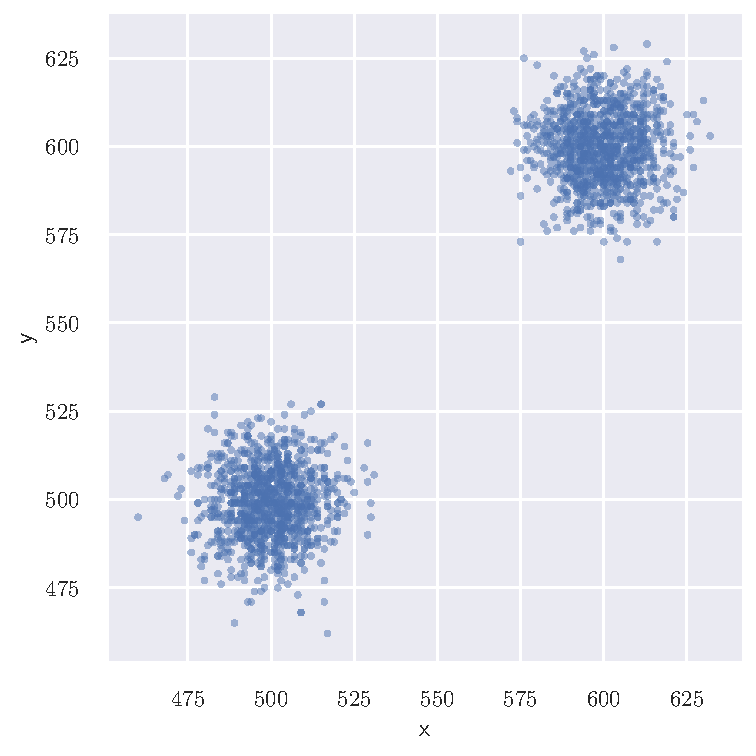
\includegraphics[width=.33\textwidth]{Figures/g2.pdf}\hfill
    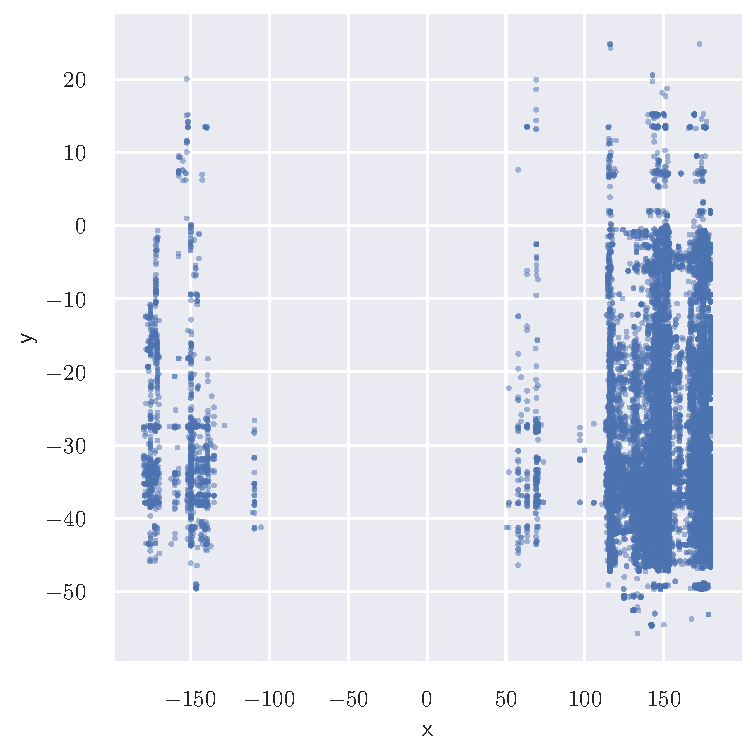
\includegraphics[width=.33\textwidth]{Figures/aus-ocean_p.pdf}
    \caption{Distribution of \texttt{post}, \texttt{g2} and \texttt{osm} datasets }\label{fig:datasets}
\end{figure}

Figure \ref{fig:datasets} illustrates the general size and distribution of each dataset. 

\textbf{Competitors}:
We are comparing LSPH with one traditional spatial index \textbf{R-Tree} \cite{Guttman:1984ka} and one learned spatial index \textbf{ZM} \cite{Wang:2019ks}

\textbf{R-Tree}: A templated C++ version implemented by Greg Douglas \cite{rtreecplus} is used for comparison. The partitioning method in this version uses the Quadratic-Cost splitting algorithm from the original R-Tree paper \cite{Guttman:1984ka}. 

\textbf{Learned ZM index}:  For the ZM model, the two-dimensional datasets convert to Z-order curve connected data. 



\section{Performance Results}

\begin{figure}
    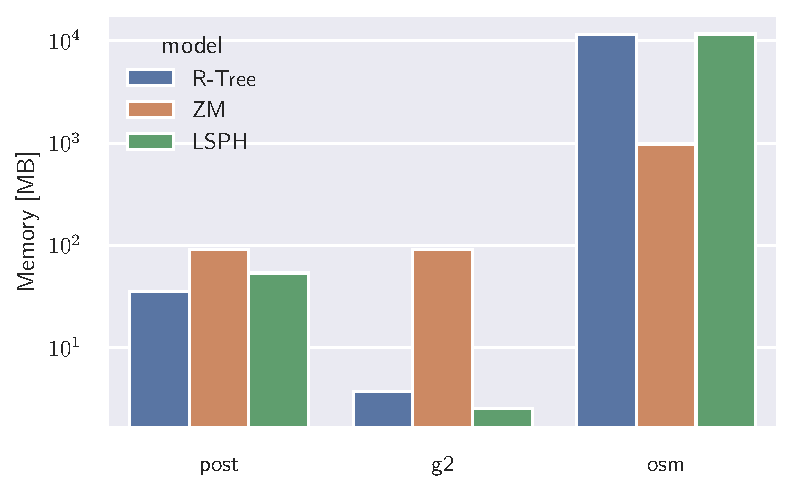
\includegraphics[width=.5\textwidth]{Figures/memory.pdf}\hfill
    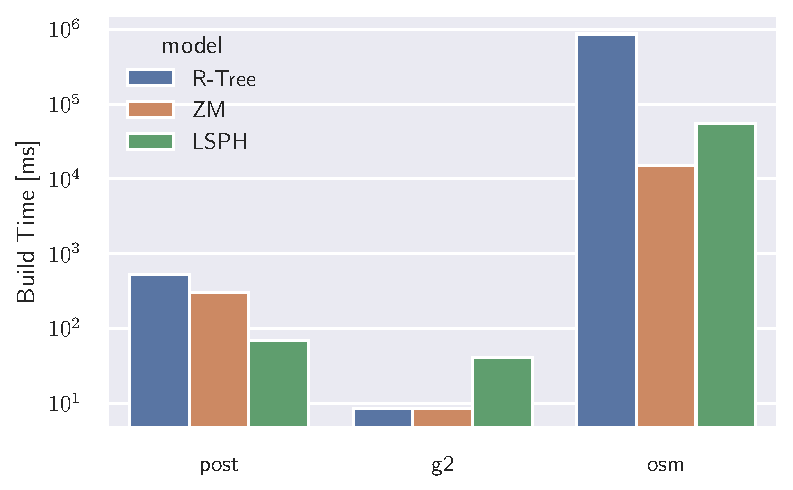
\includegraphics[width=.5\textwidth]{Figures/build_time.pdf}
    \\[\smallskipamount]
    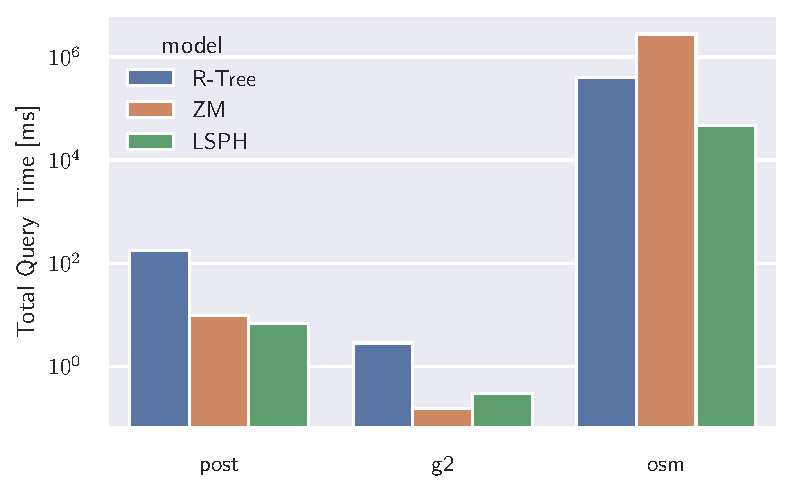
\includegraphics[width=.5\textwidth]{Figures/query_time.pdf}\hfill
    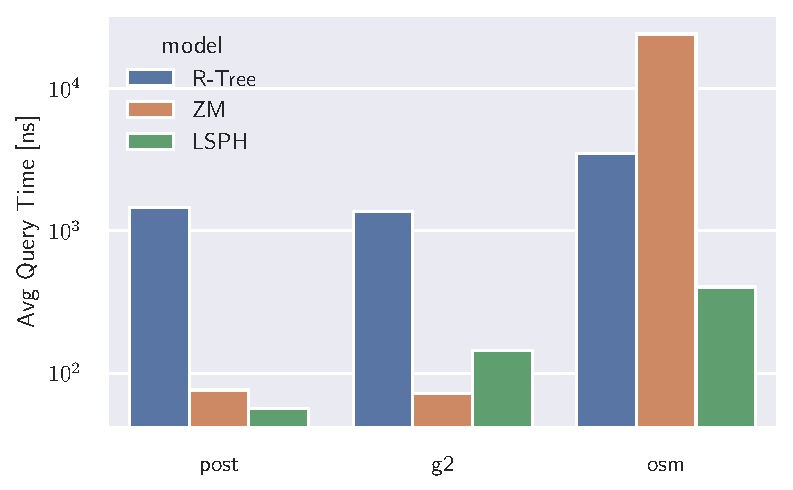
\includegraphics[width=.5\textwidth]{Figures/avg_query_time.pdf}
    \caption{Performance comparison on runtime memory, build time, total query time and average query time}\label{fig:performance}
\end{figure}

\paragraph{Runtime Memory}

\paragraph{Build Time}

\paragraph{Query Time}